\chapter{Methodology for Conducting Linear Time Reversal}
\label{ch:linear-meth}

The majority of our experiments take place within an enclosed, reflective cavity called the Gigabox: an aluminum box with a metallic foil scattering paddle to make the ray trajectories more ergodic. Ray chaos ensures that a propagating pulse will eventually reach every point in the environment, which insures that many transmission channels are simultaneously excited, and this improves reconstruction fidelity. Up to five monopole antennas inject and extract electromagnetic signals from different ports in the enclosure depending on the experiment.

Our TRM consists of three pieces of microwave processing equipment and a desktop workstation. Interrogation pulses and time-reversed sona signals are created and broadcast using a Tektronix \texttt{AWG7052} arbitrary waveform generator feeding an Agilent \texttt{E8267D} Vector PSG microwave source. A digital storage oscilloscope (DSO, Agilent \texttt{DSO91304A}) is used to record waveforms of interest. MATLAB is used for signal processing and instrument control and coordination.

In many experiments, it is necessary to be able to “read” and “write” signals from the same port. Manually switching coaxial cables from the PSG to the DSO is slow and can destroy reconstructions, so we use four HP 8762C coaxial switches to reroute signals as required.

This hardware is laid out in Figure~\ref{fig:linear-gigabox}.

\begin{figure}[h!]
\centering
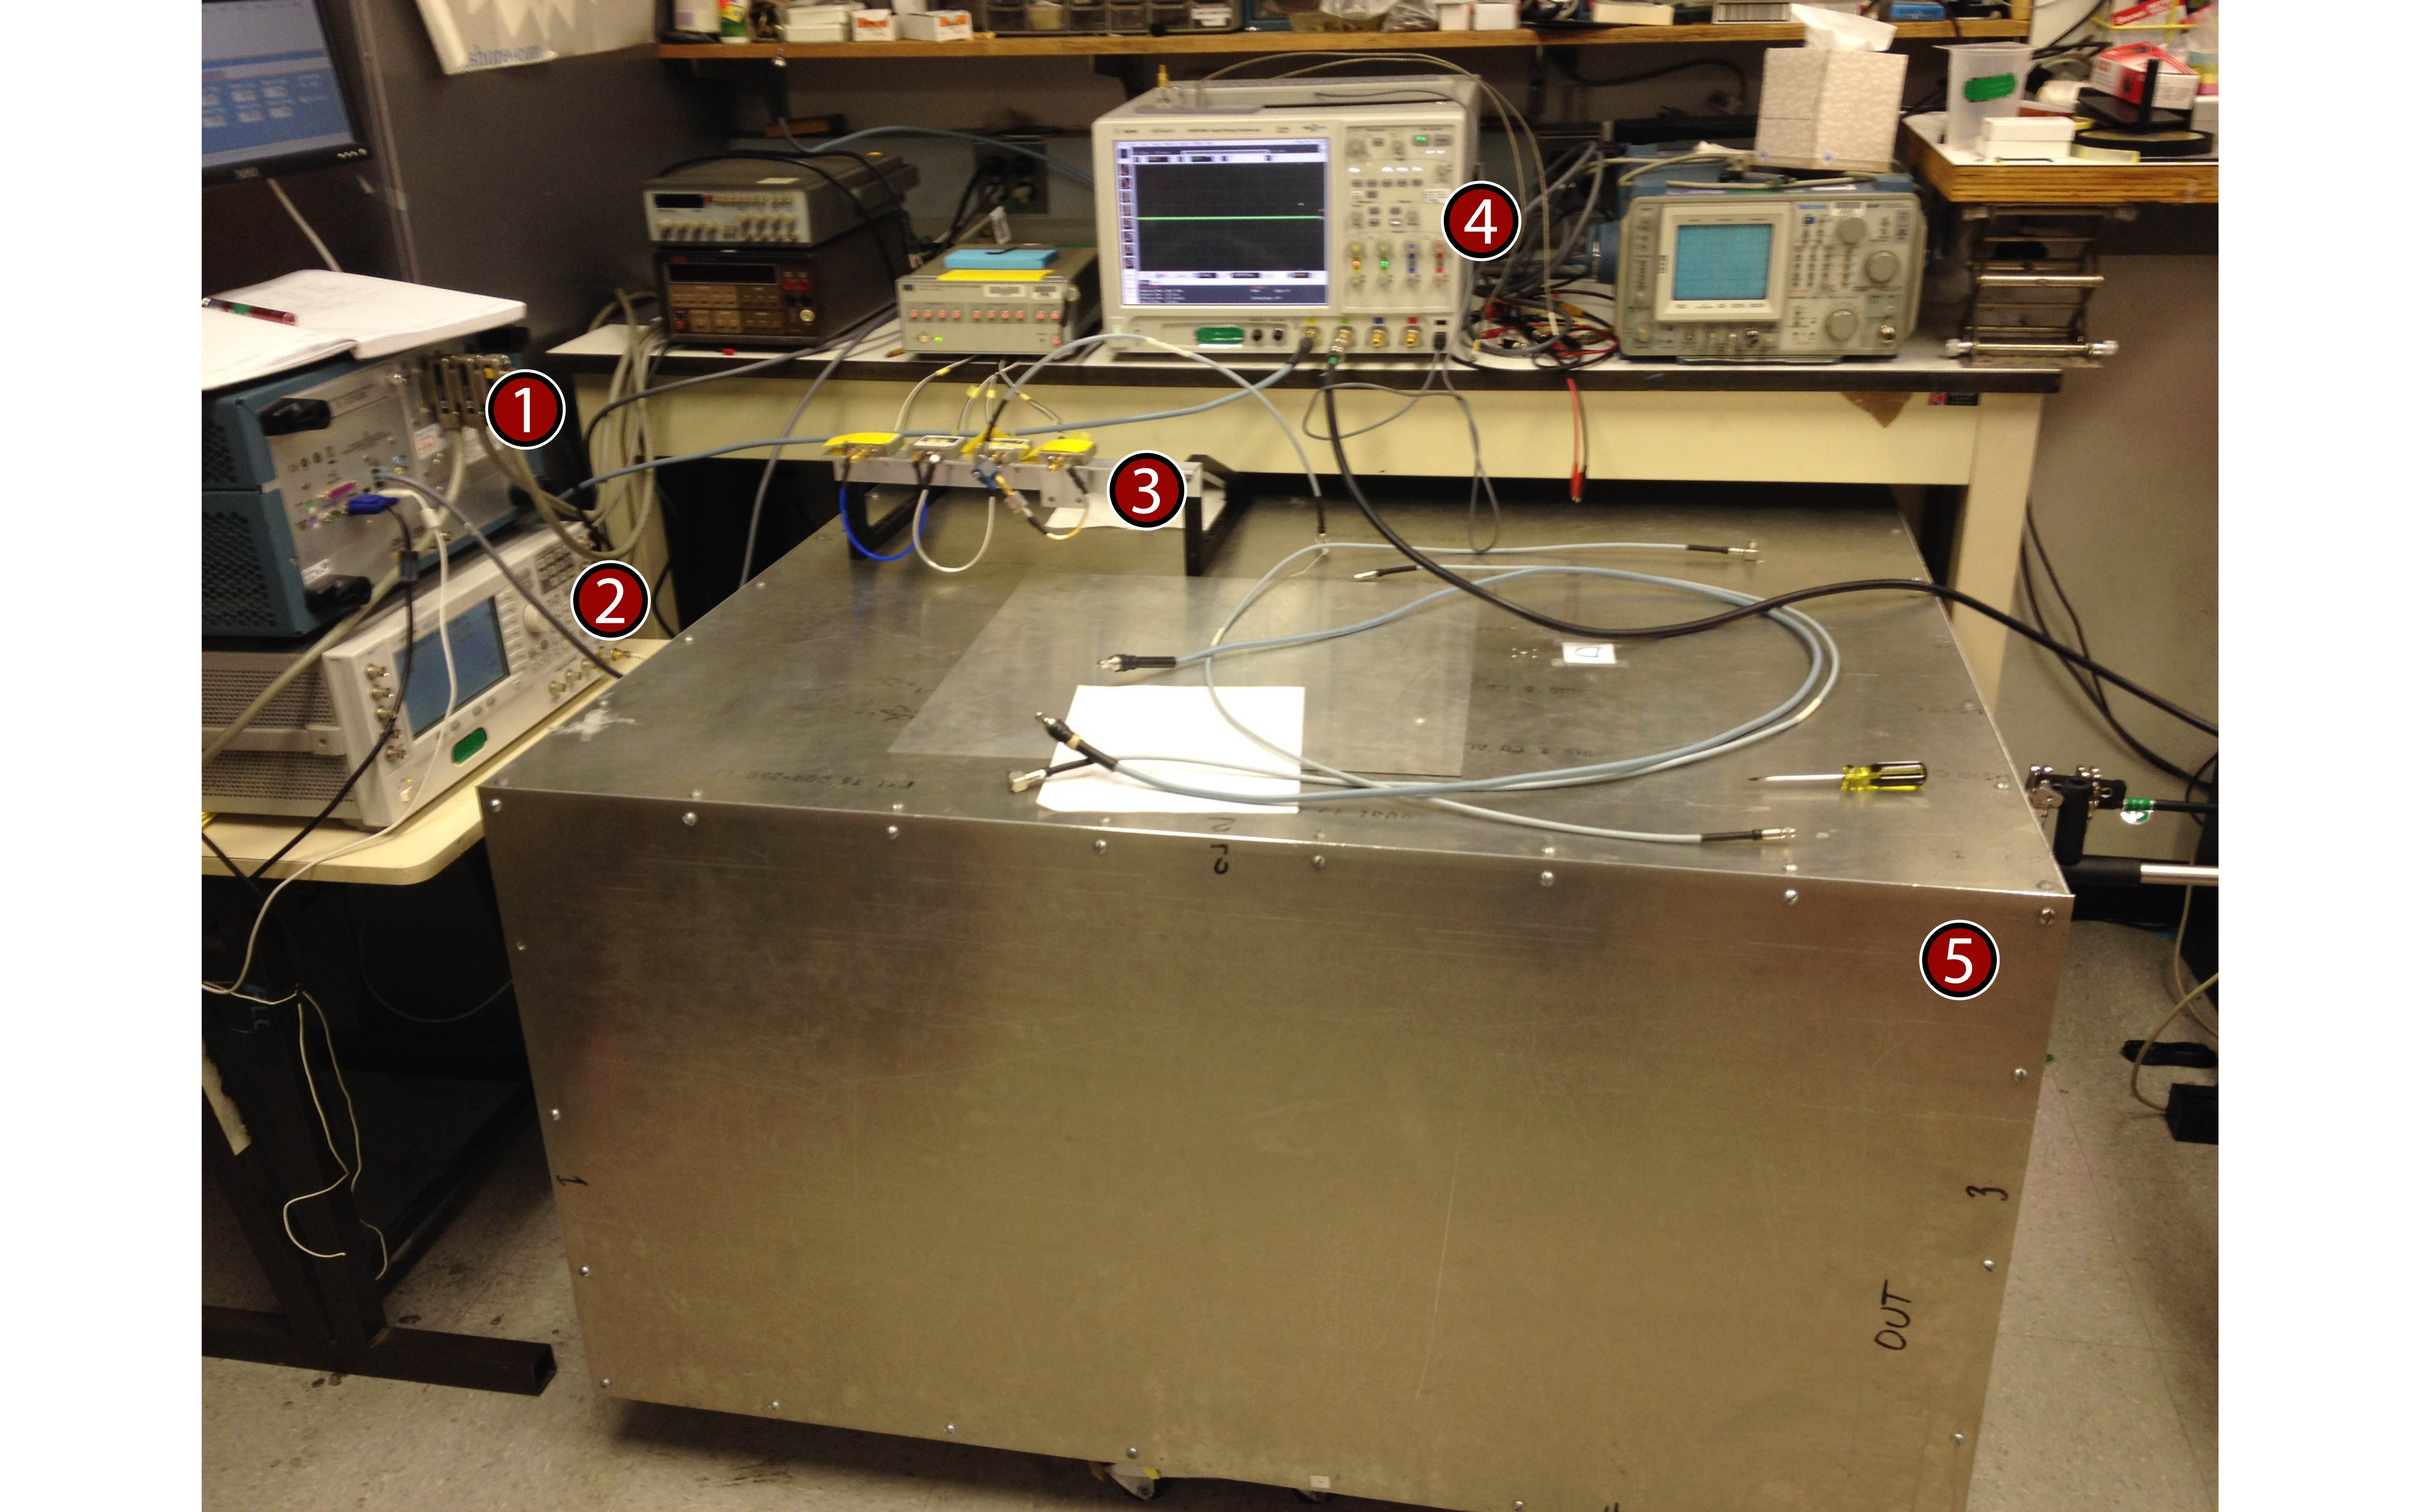
\includegraphics[width=0.85\textwidth]{linear/gigabox}
    \caption[Lab equipment setup]{Lab equipment setup: 1) Tektronix \texttt{AWG7052} Arbitrary Waveform Generator, 2) Agilent \texttt{E8267D} Vector PSG Microwave Source, 3) Array of four Hewlett-Packard 8762C coaxial switches, 4) Agilent \texttt{DSO91304A} Digital Storage Oscilloscope, 5) 1.06~$m^3$ aluminum ``Gigabox'' with interior conductive scattering paddle.}
    \label{fig:linear-gigabox}
\end{figure}

Our TR experiments fall into two main categories, which we refer to as linear and nonlinear. Nonlinear TR (or NLTR) makes use of harmonic reflections from the target to isolate it via Fourier transform after the sona is collected, a process similar to how we would envision a TR based WPT system to work. Linear TR or LTR refers to any experiment that locates the target another way, which in our case usually means taking a sona directly from the target’s location. It is experimentally much easier to get clean, strong reconstructions with LTR than with NLTR, so we use it for experiments investigating the behavior of the waves rather than the behavior of the target.

This section concerns LTR experiments. Conceptually, our general process for LTR in the Gigabox is as follows: we broadcast a Gaussian pulse from one port serving as a transmitter and collect a sona from another serving as a receiver. That sona is time reversed and rebroadcast from the transmitting port, which will cause a slightly distorted version of the original Gaussian pulse to reconstruct at the receiver. This process is illustrated in Figure~\ref{fig:linear-ltr}.


\begin{figure}[h!]
\centering
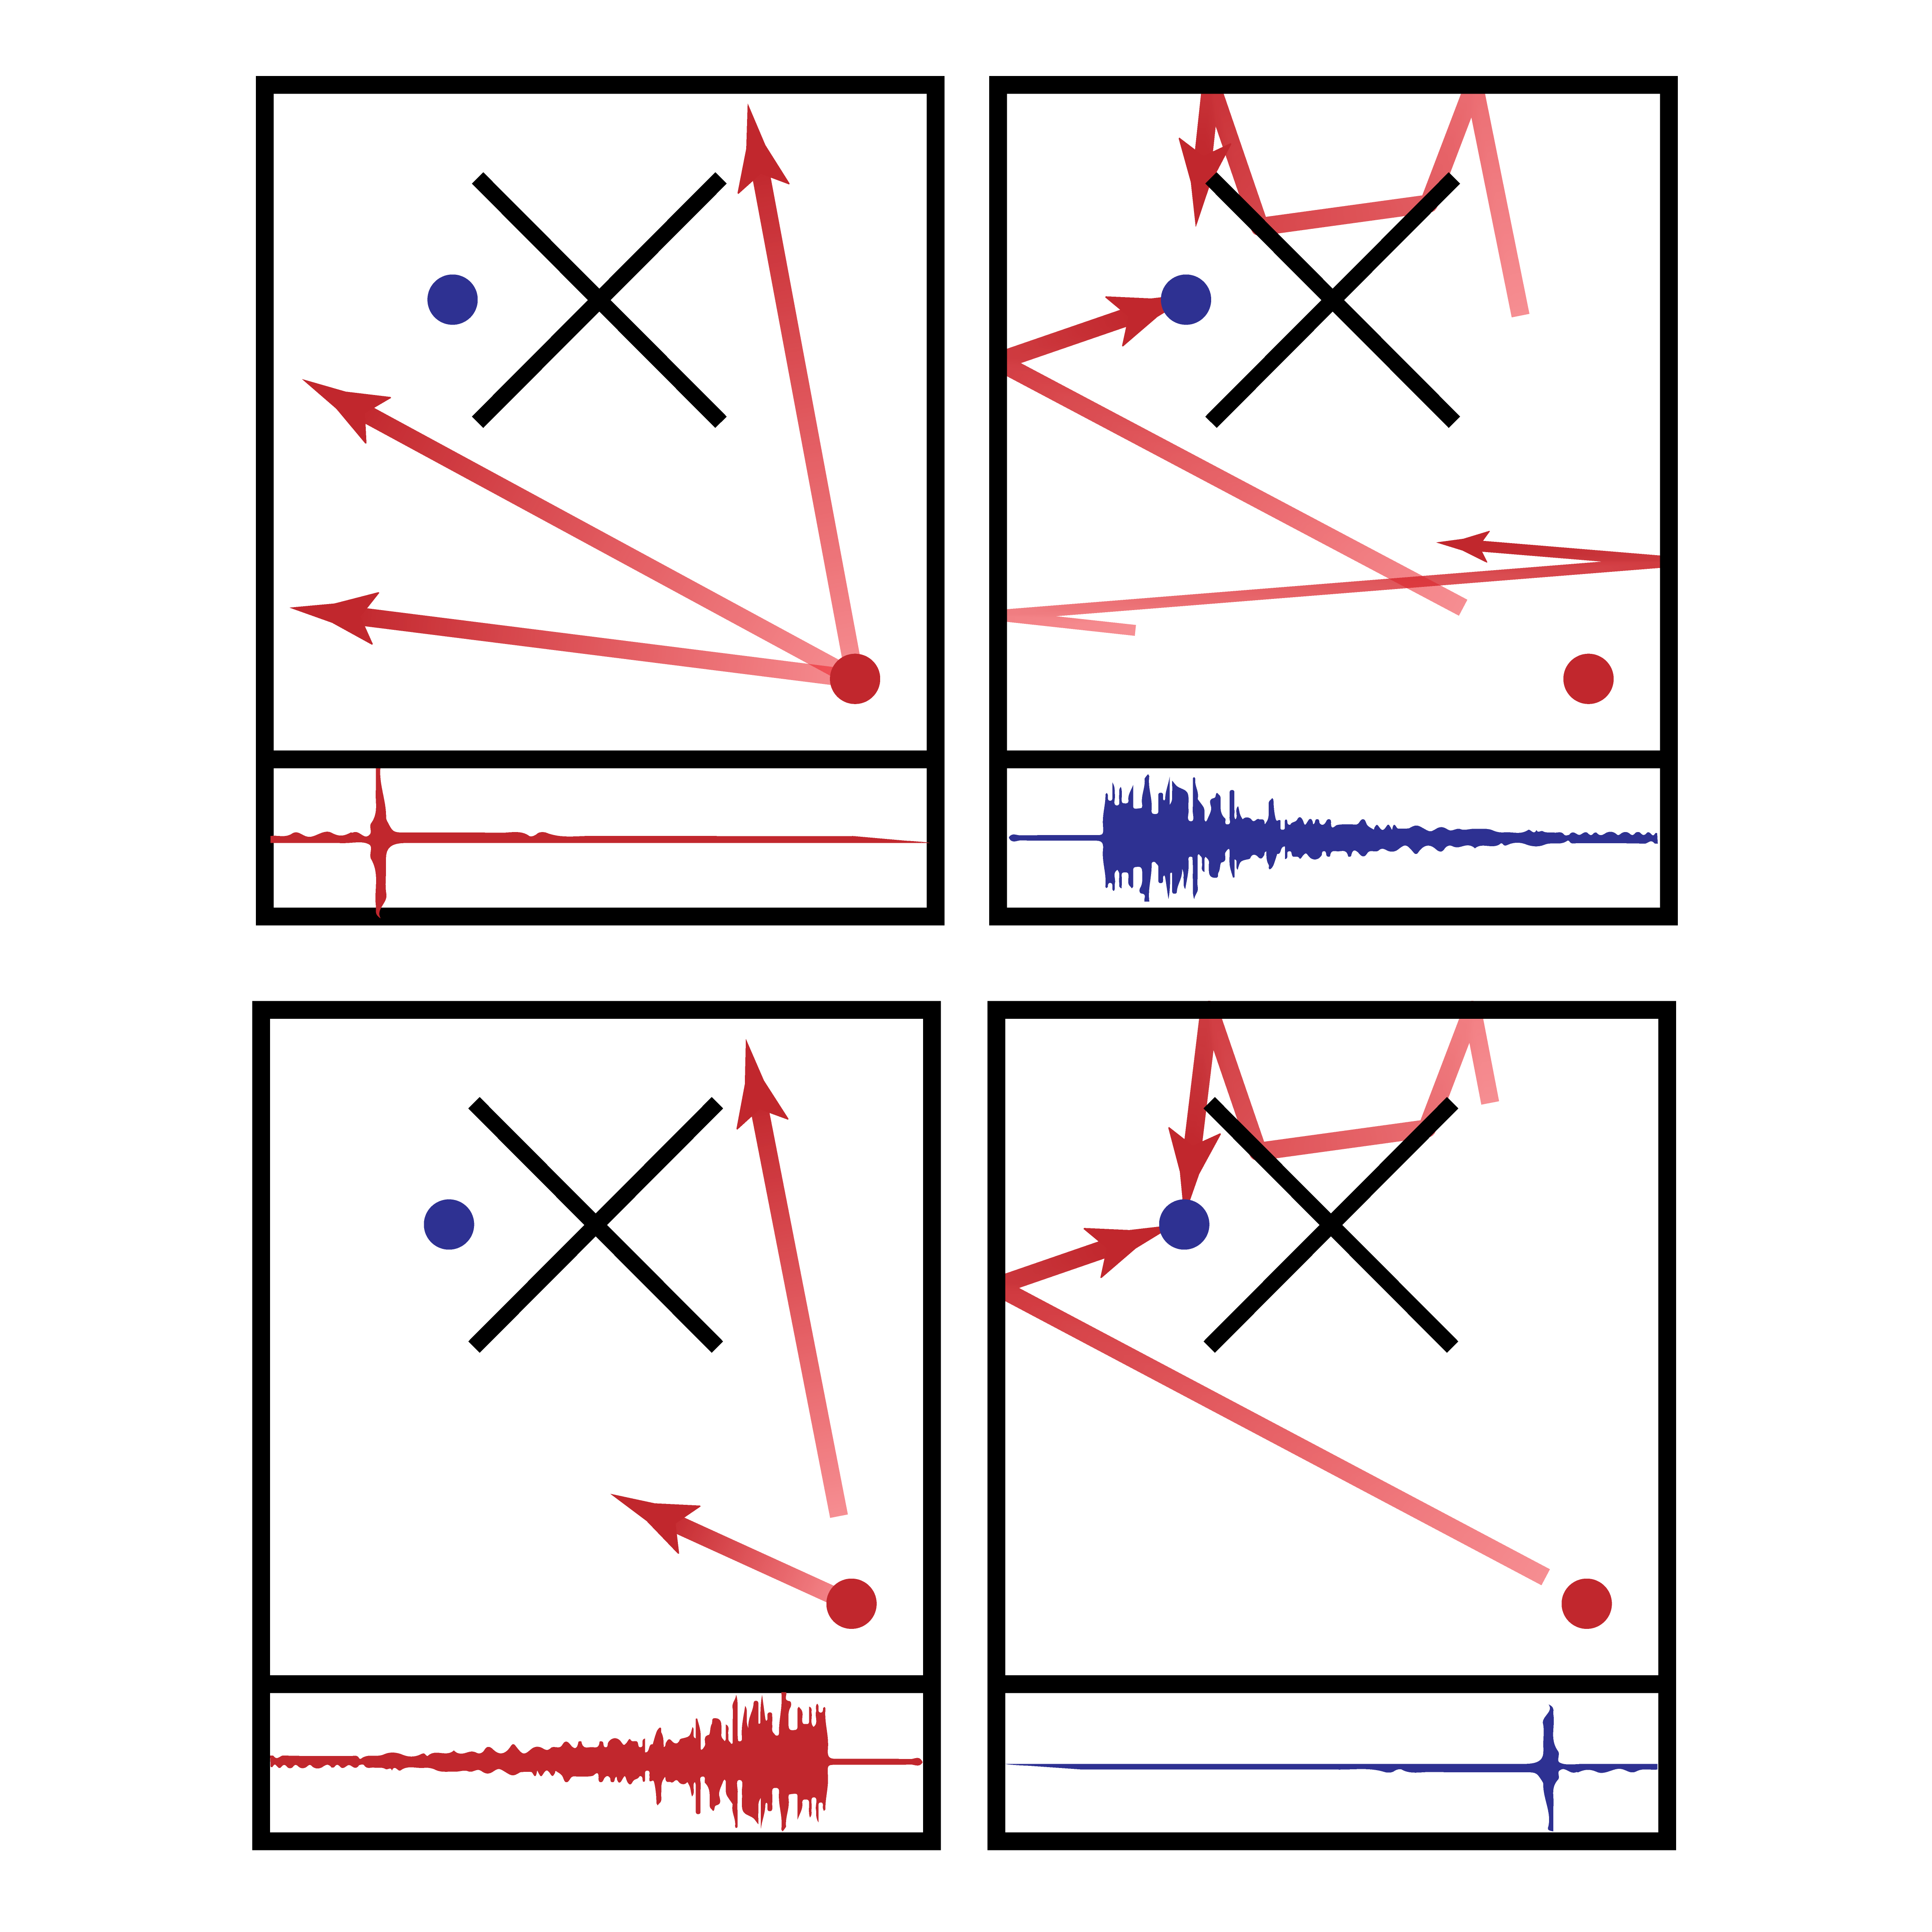
\includegraphics[width=0.85\textwidth]{linear/ltr}
    \caption[ltr]{Reading order from top left: 1) The TRM broadcasts a signal (in this case, a pulse, pictured in the inset below the panel) into the cavity, which 2) reverberates within the cavity. Some of the reflections incoherently reach the receiver as the sona, represented in blue in the inset. 3) The TRM time reverses the sona, then re-emits it into the cavity. 4) The time reversed waves coherently collapse back on the receiver in a slightly distorted reconstruction of the original pulse (inset, blue).}
    \label{fig:linear-ltr}
\end{figure}

\todo{OUGHT TO HAVE AN OUTRO HERE}